% Two full-page comparison figures copied from the verified nine-seed output.
\clearpage
\begingroup
\newgeometry{layoutwidth=11in,layoutheight=8.5in,margin=0.5in}
\paperwidth=11in\paperheight=8.5in
\ifdefined\pdfpagewidth\pdfpagewidth=\paperwidth\pdfpageheight=\paperheight
\else\ifdefined\pagewidth\pagewidth=\paperwidth\pageheight=\paperheight
\else\special{papersize=11in,8.5in}\fi\fi
\captionsetup{font=small}
\centering
\noindent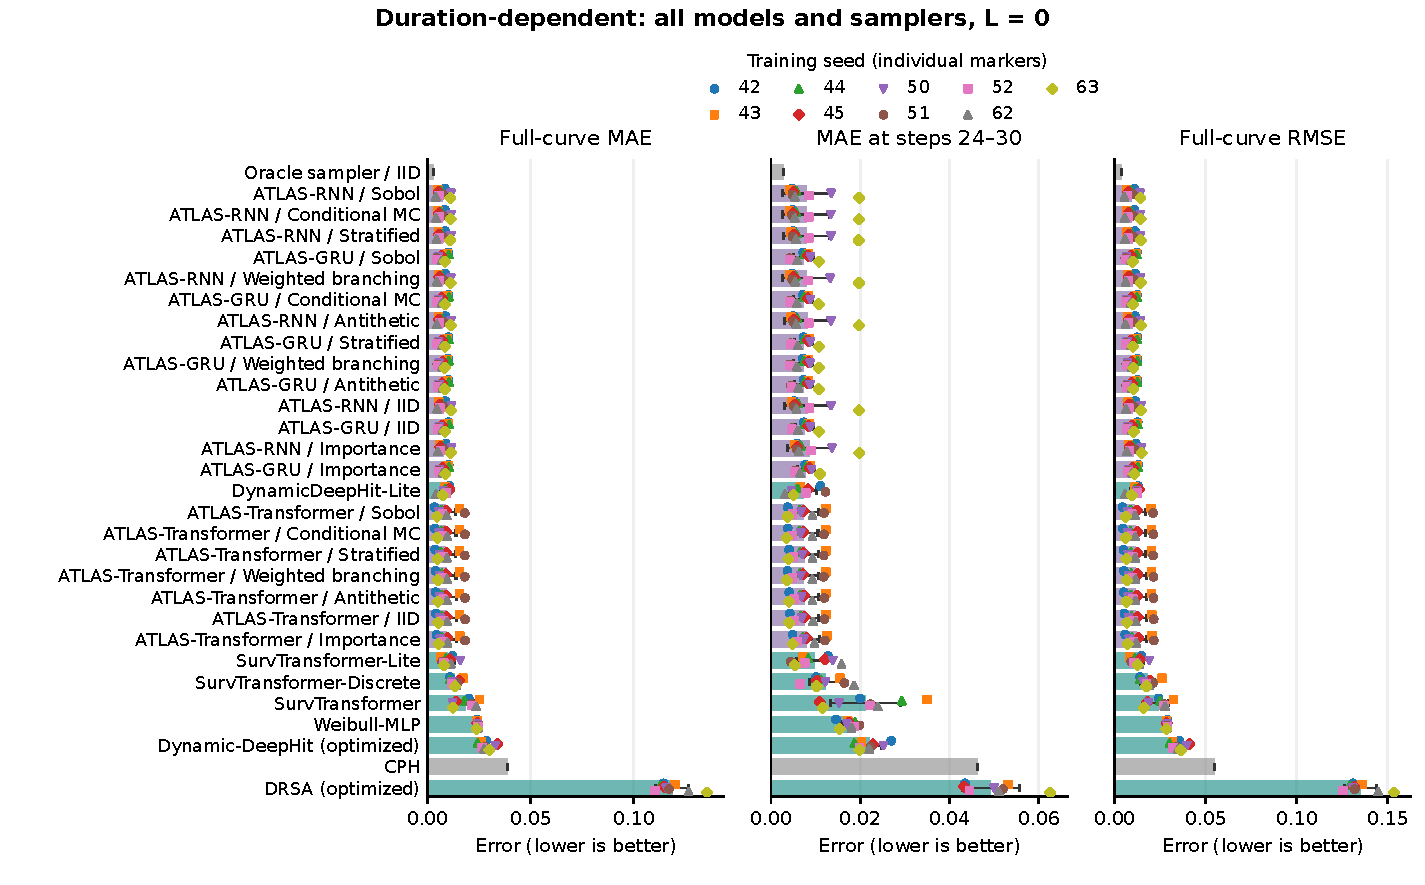
\includegraphics[width=0.95\linewidth,height=0.80\textheight,keepaspectratio]{hard24_nine_seed_comparison_L0.pdf}\par
\captionof{figure}{Nine-training-run comparison at $L=0$ in the single-covariate duration-dependent experiment. The panels show full-curve MAE, MAE restricted to steps 24--30, and RMSE. Bars are means over training runs; colored markers show individual runs and error bars show their standard deviation. Each stochastic training-run score averages five sampling seeds at $M=10{,}000$. CPH and the true-generator oracle are unchanged controls, shown from the seed-42 source without training-variation error bars. Dynamic-DeepHit (optimized) and DRSA (optimized) use the validation-selected fits, and row order follows the updated mean survival MAE. Lower error is better.}\label{fig:hard24_nine_L0}\par
\clearpage
\noindent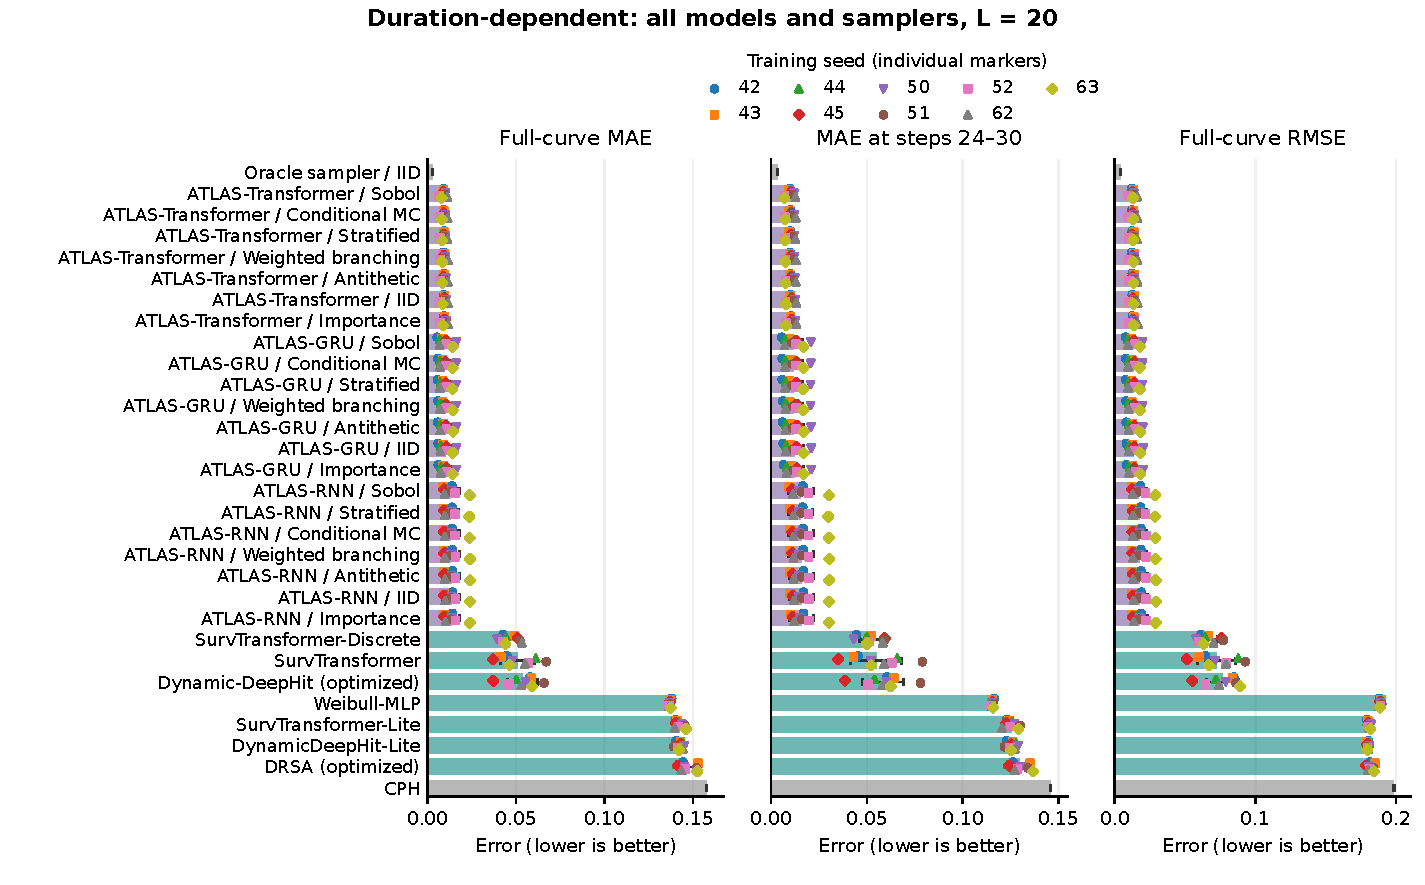
\includegraphics[width=0.95\linewidth,height=0.80\textheight,keepaspectratio]{hard24_nine_seed_comparison_L20.pdf}\par
\captionof{figure}{Nine-training-run comparison at $L=20$ in the single-covariate duration-dependent experiment. The panels show full-curve MAE, MAE restricted to steps 24--30, and RMSE. Bars are means over training runs; colored markers show individual runs and error bars show their standard deviation. Each stochastic training-run score averages five sampling seeds at $M=10{,}000$. CPH and the true-generator oracle are unchanged controls, shown from the seed-42 source without training-variation error bars. Dynamic-DeepHit (optimized) and DRSA (optimized) use the validation-selected fits, and row order follows the updated mean survival MAE. Lower error is better.}\label{fig:hard24_nine_L20}\par
\clearpage
\restoregeometry
\paperwidth=8.5in\paperheight=11in
\ifdefined\pdfpagewidth\pdfpagewidth=\paperwidth\pdfpageheight=\paperheight
\else\ifdefined\pagewidth\pagewidth=\paperwidth\pageheight=\paperheight
\else\special{papersize=8.5in,11in}\fi\fi
\endgroup
